% ft-10-ProductQuotient.tex

\documentclass[xcolor=dvipsnames]{beamer}

\usepackage{cancel}
\renewcommand{\CancelColor}{\color{red}}
\usepackage{graphicx}
\usepackage{wrapfig}
\usepackage{colortbl}
\usepackage{color}
\usepackage{alltt}
\renewcommand*{\thefootnote}{\fnsymbol{footnote}}
\definecolor{myblue}{rgb}{0.8,0.85,1}

\mode<presentation>
{
  \usetheme{Warsaw}
  \setbeamercovered{transparent}
}
% \usecolortheme[named=OliveGreen]{structure}
\setbeamertemplate{navigation symbols}{} 
\setbeamertemplate{blocks}[rounded][shadow=true] 

% this is for overlaying math symbols, see https://tex.stackexchange.com/questions/12895/overlay-symbol-with-another
\def\qeq{\mathrel{%
    \mathchoice{\QEQ}{\QEQ}{\scriptsize\QEQ}{\tiny\QEQ}%
}}
\def\QEQ{{%
    \setbox0\hbox{$\longrightarrow$}%
    \rlap{\hbox to \wd0{\hss/\hss}}\box0
  }}

\newcounter{expls}
\setcounter{expls}{0}
\newcommand{\beispiel}[1]{\refstepcounter{expls}\textbf{Example \arabic{expls}: #1.}}

\newcounter{exercise}
\setcounter{exercise}{0}
\newcommand{\ubung}[0]{\refstepcounter{exercise}\textbf{Exercise \arabic{exercise}: }}

\newif\ifBCITCourse
\BCITCoursetrue
% \BCITCoursefalse
\newif\ifWhichCourse
\WhichCoursetrue
% \WhichCoursefalse
\ifBCITCourse
\ifWhichCourse
\newcommand{\CourseName}{Technical Mathematics for Food Technology}
\newcommand{\CourseNumber}{MATH 1441}
\newcommand{\CourseInst}{BCIT}
\else
\newcommand{\CourseName}{Technical Mathematics for Geomatics}
\newcommand{\CourseNumber}{MATH 1511}
\newcommand{\CourseInst}{BCIT}
\fi
\else
\newcommand{\CourseName}{Philosophy and Literature}
\newcommand{\CourseNumber}{PHIL 375}
\newcommand{\CourseInst}{UBC}
\fi

\title{Product and Quotient Rule}
\subtitle{{\CourseNumber}, BCIT}

\author{\CourseName}

\date{November 2, 2017}

\begin{document}

\begin{frame}
  \titlepage
\end{frame}

\begin{frame}
  \frametitle{Product Rule}
  \begin{block}{Rule 5}
The Product Rule
  \end{block}
\begin{equation}
  \label{eq:aepuaxai}
g'(x)=f_{1}(x)f_{2}'(x)+f_{1}'(x)f_{2}(x)\mbox{ for }g(x)=f_{1}(x)f_{2}(x)
\end{equation}
\end{frame}

\begin{frame}
  \frametitle{Product Rule Reason}
Reason:
\begin{equation}
  \label{eq:yahtiera}
g'(x)=\notag
\end{equation}
\begin{equation}
  \label{eq:piebaith}
\lim_{h\rightarrow{}0}\frac{g(x+h)-g(x)}{h}=\lim_{h\rightarrow{}0}\frac{f_{1}(x+h)f_{2}(x+h)-f_{1}(x)f_{2}(x)}{h}=\notag
\end{equation}
\begin{equation}
  \label{eq:eceishie}
\lim_{h\rightarrow{}0}\frac{f_{1}(x+h)f_{2}(x+h)\alert{-f_{1}(x)f_{2}(x+h)+f_{1}(x)f_{2}(x+h)}-f_{1}(x)f_{2}(x)}{h}=\notag
\end{equation}
\begin{equation}
  \label{eq:chiekeey}
\lim_{h\rightarrow{}0}\frac{(f_{1}(x+h)-f_{1}(x))f_{2}(x+h)+f_{1}(x)(f_{2}(x+h)-f_{2}(x))}{h}=\notag
\end{equation}
\begin{equation}
  \label{eq:vaeyiewe}
f_{1}(x)f_{2}'(x)+f_{1}'(x)f_{2}(x)
\end{equation}
\end{frame}

\begin{frame}
  \frametitle{Product Rule Exercises}
{\ubung} Differentiate the following functions.
\begin{equation}
  \label{eq:iefeiwah}
f(x)=(2x^{2}-1)(x^{3}+3)
\end{equation}
\begin{equation}
  \label{eq:recootie}
g(t)=t^{3}\left(\sqrt{t}+1\right)
\end{equation}
\end{frame}

\begin{frame}
  \frametitle{Quotient Rule}
  \begin{block}{Rule 6}
The Quotient Rule
  \end{block}
\begin{equation}
  \label{eq:roothubu}
g'(x)=\frac{f_{1}'(x)f_{2}(x)-f_{1}(x)f_{2}'(x)}{\left(f_{2}(x)\right)^{2}}\mbox{ for }g(x)=\frac{f_{1}(x)}{f_{2}(x)}
\end{equation}
\end{frame}

\begin{frame}
  \frametitle{Quotient Rule Reason}
Reason:
\begin{equation}
  \label{eq:iebowohc}
g(x)=\frac{f_{1}(x)}{f_{2}(x)}
\end{equation}
\begin{equation}
  \label{eq:iilahthi}
f_{1}(x)=g(x)f_{2}(x)
\end{equation}
\begin{equation}
  \label{eq:eshohhoo}
f_{1}'(x)=g'(x)f_{2}(x)+g(x)f_{2}'(x)\mbox{ now isolate }g'(x)
\end{equation}
\begin{equation}
  \label{eq:iophiewu}
g'(x)=\frac{f_{1}'(x)-g(x)f_{2}'(x)}{f_{2}(x)}\mbox{ now substitute }g(x)=\frac{f_{1}(x)}{f_{2}(x)}
\end{equation}
\begin{equation}
  \label{eq:uhushain}
g'(x)=\frac{\frac{f_{1}'(x)f_{2}(x)}{f_{2}(x)}-\frac{f_{1}(x)f_{2}'(x)}{f_{2}(x)}}{f_{2}(x)}
\end{equation}
\begin{equation}
  \label{eq:requuare}
g'(x)=\frac{f_{1}'(x)f_{2}(x)-f_{1}(x)f_{2}'(x)}{\left(f_{2}(x)\right)^{2}}
\end{equation}
\end{frame}

\begin{frame}
  \frametitle{Quotient Rule Exercises}
{\ubung} Differentiate the following functions.
\begin{equation}
  \label{eq:xookaeji}
f(z)=\frac{3z^{2}+5z-2}{3z-1}
\end{equation}
\begin{equation}
  \label{eq:eidoogow}
h(x)=\frac{\sqrt{x}}{x^{2}+1}
\end{equation}
\end{frame}

\begin{frame}
  \frametitle{Quotient Rule Exercise Solution}
  \begin{figure}[h]
    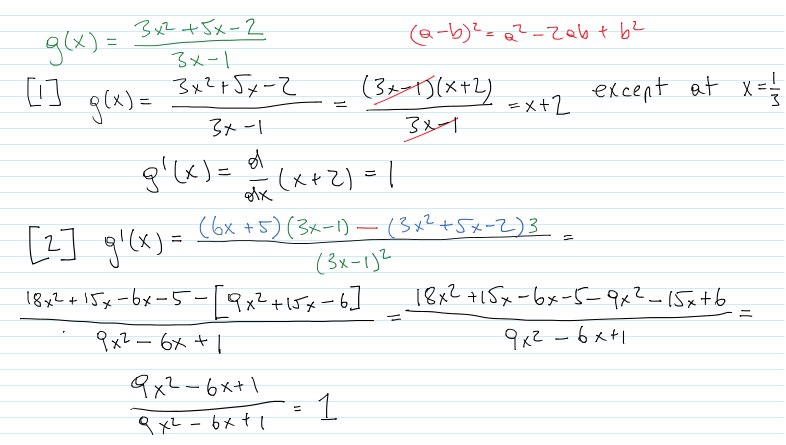
\includegraphics[scale=0.575]{./onenote_ft_09_ProductQuotientRule_02.png}
  \end{figure}
\end{frame}

\begin{frame}
  \frametitle{Euler's Number}
The number $e$ is defined as follows,
\begin{equation}
  \label{eq:ciedaeme}
  e=\lim_{t\rightarrow\infty}\left(1+\frac{1}{t}\right)^{t}
\end{equation}
\end{frame}

\begin{frame}
  \frametitle{Lemma}
Consider two functions $f_{1}$ and $f_{2}$. They are related in so far
as
\begin{equation}
  \label{eq:ohquailo}
  f_{1}(x)=f_{2}\left(\frac{1}{x}\right)
\end{equation}
For example,
\begin{equation}
  \label{eq:seemaxah}
  f_{1}(x)=\frac{2x+1}{5x-7}\mbox{ and }f_{2}(x)=-\frac{x+2}{7x-5}
\end{equation}
Then
\begin{equation}
  \label{eq:iebieluk}
  \mbox{If }\lim_{x\rightarrow\infty}f_{1}(x)=a\mbox{ then }\lim_{x\rightarrow{}0}f_{2}(x)=a
\end{equation}
\end{frame}

\begin{frame}
  \frametitle{The Derivative of the Logarithmic Function}
Now consider the function $f(x)=\ln{}x$ and the definition of the
derivative,
\begin{equation}
  \label{eq:eeghaphe}
  f'(x)=\lim_{h\rightarrow{}0}\frac{f(x+h)-f(x)}{h}=\lim_{h\rightarrow{}0}\frac{1}{h}\ln\frac{x+h}{x}=\notag
\end{equation}
\begin{equation}
  \label{eq:quanoefe}
  \lim_{h\rightarrow{}0}\frac{1}{x}\cdot\frac{x}{h}\ln\left(1+\frac{h}{x}\right)=\lim_{h\rightarrow{}0}\frac{1}{x}\ln\left(1+\frac{1}{\frac{x}{h}}\right)^{\frac{x}{h}}
\end{equation}
Use the lemma of the last slide and the definition of Euler's number to see that
\begin{equation}
  \label{eq:oozeexei}
  f'(x)=\frac{1}{x}
\end{equation}
\end{frame}

\begin{frame}
  \frametitle{Exercises}
  {\ubung} Differentiate the following functions.
  \begin{equation}
    \label{eq:eipovaif}
    f(x)=x^{2}\ln{}x
  \end{equation}
  \begin{equation}
    \label{eq:ejahshai}
    g(y)=\ln{}y^{(5y-2)}
  \end{equation}
  \begin{equation}
    \label{eq:nooshahw}
    h(z)=\left(\ln{}z\right)^{2}
  \end{equation}
  \begin{equation}
    \label{eq:weeshieb}
    f(x)=\log_{2}x
  \end{equation}
\end{frame}

\begin{frame}
  \frametitle{End of Lesson}
Next Lesson: Chain Rule
\end{frame}

\end{document}

